

\chapter{Introduction}

\pagenumbering{arabic}
\setcounter{page}{2}
%\noindent
%\parindent=0cm

%${\mathcal{C}}_{53}$\\
%$\overline{\mathcal{C}}_{53}$\\
%${\mathcal{PC}}_{53}$\\

Le but de ce document est de démontrer que quatre couleurs suffisent pour colorier n'importe quelle carte géographique et dès lors que tout graphe simple, planaire et connexe est de nombre chromatique quatre (voir la section suivante pour la définition de ces critères). Ce résultat est connu sous le nom du \textit{théorème des quatre couleurs}.\bigskip

Le problème remonte à 1852, lorsque le cartographe anglais Francis \textsc{Guthrie} remarqua qu'il lui suffisait de quatre couleurs pour colorer la carte (pourtant complexe) des comtés d'Angleterre, sans que deux cantons voisins ne reçoivent la même couleur. Son frère Frederick, mathématicien, ne parvenant pas à savoir si la propriété était générale, transmit la réflexion à son professeur, Auguste \textsc{de Morgan} de la \textit{University College} de Londres. Et de fil en aiguille, le problème (devenu postulat, puis conjecture), se répandit dans la sphère mathématique, aidé en 1978 par la publication de la question par Arthur \textsc{Cayley} et son évocation lors d'un colloque de la \textit{London Mathematical Society}. Prèsqu'aussitôt, Alfred \textsc{Kempe} propose une preuve de la conjecture en 1879 et, pendant une décennie, on crut le problème des quatre couleurs résolu. \textsc{Kempe} fut élu membre de la \textit{Royal Society} et devint ensuite président de la \textit{London Mathematical Society}. Mais onze ans plus tard, en 1890, Percy John \textsc{Heawood} trouva une faille majeure dans la démonstration. Il parvient cependant à sauvegarder tant bien que mal la preuve en un \textit{théorème des cinq couleurs}. Une seconde preuve, proposée par Peter Guthrie \textsc{Tait} dès 1880, fut également réfutée, par Julius \textsc{Peterson} en 1891.\smallskip

De nombreuses tentatives ont étés introduites pour réduire à quatre le nombre de couleurs à partir de la démonstration de \textsc{Kempe-Heawood}. En 1913, le père de l'algèbre moderne George David \textsc{Birkhoff}, formule une notion de configuration réductible et démontre la conjecture pour toutes les cartes comportant moins de vingt-six régions à colorier et cette borne est petit à petit améliorée au cours du siècle. En 1969, Heinrich \textsc{Heesch} trouve des conditions \textit{presque} nécessaires et suffisantes pour qu'une configuration soit réductible et une méthode générale pour trouver un ensemble de configurations inévitable. Ce n'est finalement qu'en 1976 que la première démonstration complète fut acceptée, celle de Kenneth \textsc{Appel} et Wolfgang \textsc{Haken}. Ces derniers réalisèrent de manière informatique le programme de \textsc{Heesch} et montrèrent, après 1200 heures de calcul et des dizaines de milliers de figures à l'appui, que les 1478 configurations sont réductibles et 4-coloriables. Cette preuve fut la première démonstration acceptée sur base de l'utilisation massive de l'ordinateur. Enfin, en 1995, Neil \textsc{Robertson}, Daniel \textsc{Sanders}, Paul \textsc{Seymour} et Robin \textsc{Thomas} mirent à profit l'avancement de la technologie pour compiler une réalisation nettement plus simple du programme de \textsc{Heesch}, avec seulement 633 configurations.

Dans ce document, nous déclarons exposer une preuve complète du théorème qui ne nécessite pas l'utilisation d'outil informatique.

Notre document est découpé en 3 chapitres.\\
Dans le 1er chapitre, nous donnons les définitions permettant de cadrer notre propos et tout particulièrement la définition du graphe géographique et de la chaine de Kempe.
Dans le 2ème chapitre nous reprenons la démonstration du théorème des cinq couleurs. Ce n'est pas directement notre sujet, mais nous nous basons sur les mêmes principes, il était donc normal de les rappeler. Enfin, le 3ème chapitre s’attaque au théorème des quatre couleurs et à sa résolution.

\section{Carte et coloration}

Pour colorer une carte géographique, on demande que toute paire de pays limitrophes soit coloriée de deux couleurs différentes afin de visualiser clairement la frontière qui sépare les deux pays. Dans le cadre de la démonstration du théorème, nous ne considérerons que des pays connexes, c'est-à-dire constitués d'un seul morceau\footnote{La Corse, l'Alaska ou Baerle-Duc sont dès lors considérés comme des pays indépendants.}. De plus, nous restreindrons la définition de frontière entre deux pays à des courbes de longueur non nulle : deux pays ne se touchant que par un point ne sont pas considérés comme limitrophes. Enfin, nous considérerons que la carte étudiée est constituée d'un nombre fini de pays, regroupés en un ensemble connexe unique (\textit{i.e.}~ nous ne regardons qu'un seul continent).

À toute carte géographique satisfaisant ces hypothèses, on peut associer un \textit{graphe} coloré\footnote{Une coloration d'un graphe $G$ est une fonction associant à tout sommet de $G$ une couleur, généralement un élément de l'ensemble d'indices $\{1, 2, ..., n\}$, telle que deux sommets adjacents n'ont pas la même couleur (où $n$ est le nombre de sommets du graphe). De manière équivalente, en définissant un \textit{stable} de \textit{G} par un sous-ensemble de sommets deux-à-deux non adjacents, une coloration de $G$ est une partition de son ensemble de sommets en stables. On ne différentie généralement pas les colorations qui ne sont distinctes qu'à une permutation des indices de couleurs près.}, c'est-à-dire une représentation schématique des liens entre les pays (voir Figure~\ref{Carte}). Chaque pays est représenté par un \textit{sommet} coloré, relié par des \textit{arrêtes} à ses pays limitrophes. Le nombre de pays limitrophes à un sommet (\textit{i.e.}~le nombre d'arêtes partant de ce sommet) est appelé son \textit{degré}, que l'on note~$d\in\mathbb{N}^+$. Les polygones délimités par les arrêtes entre les sommets sont appelés les \textit{faces} du graphe\footnote{Les équivalents de ces faces dans la carte géographique d'origine pourraient être appelés des \textit{embranchement de frontières}, c'est à dire des points d'où partent au moins trois frontières ou, dit autrement, où au moins trois pays se rencontrent. Ce n'est cependant pas toujours vrai : sur le graphe de la Figure~\ref{Carte} le Liechtenstein et l'Allemagne bordent la même face alors qu'ils ne partagent pas de frontière.}. Précisons tout de suite que l'espace externe délimité par le graphe est toujours considéré comme étant une face\footnote{Un graphe ne comportant qu'un seul sommet et aucune arête possède donc une face.}.

\begin{figure}[b!]\centering{
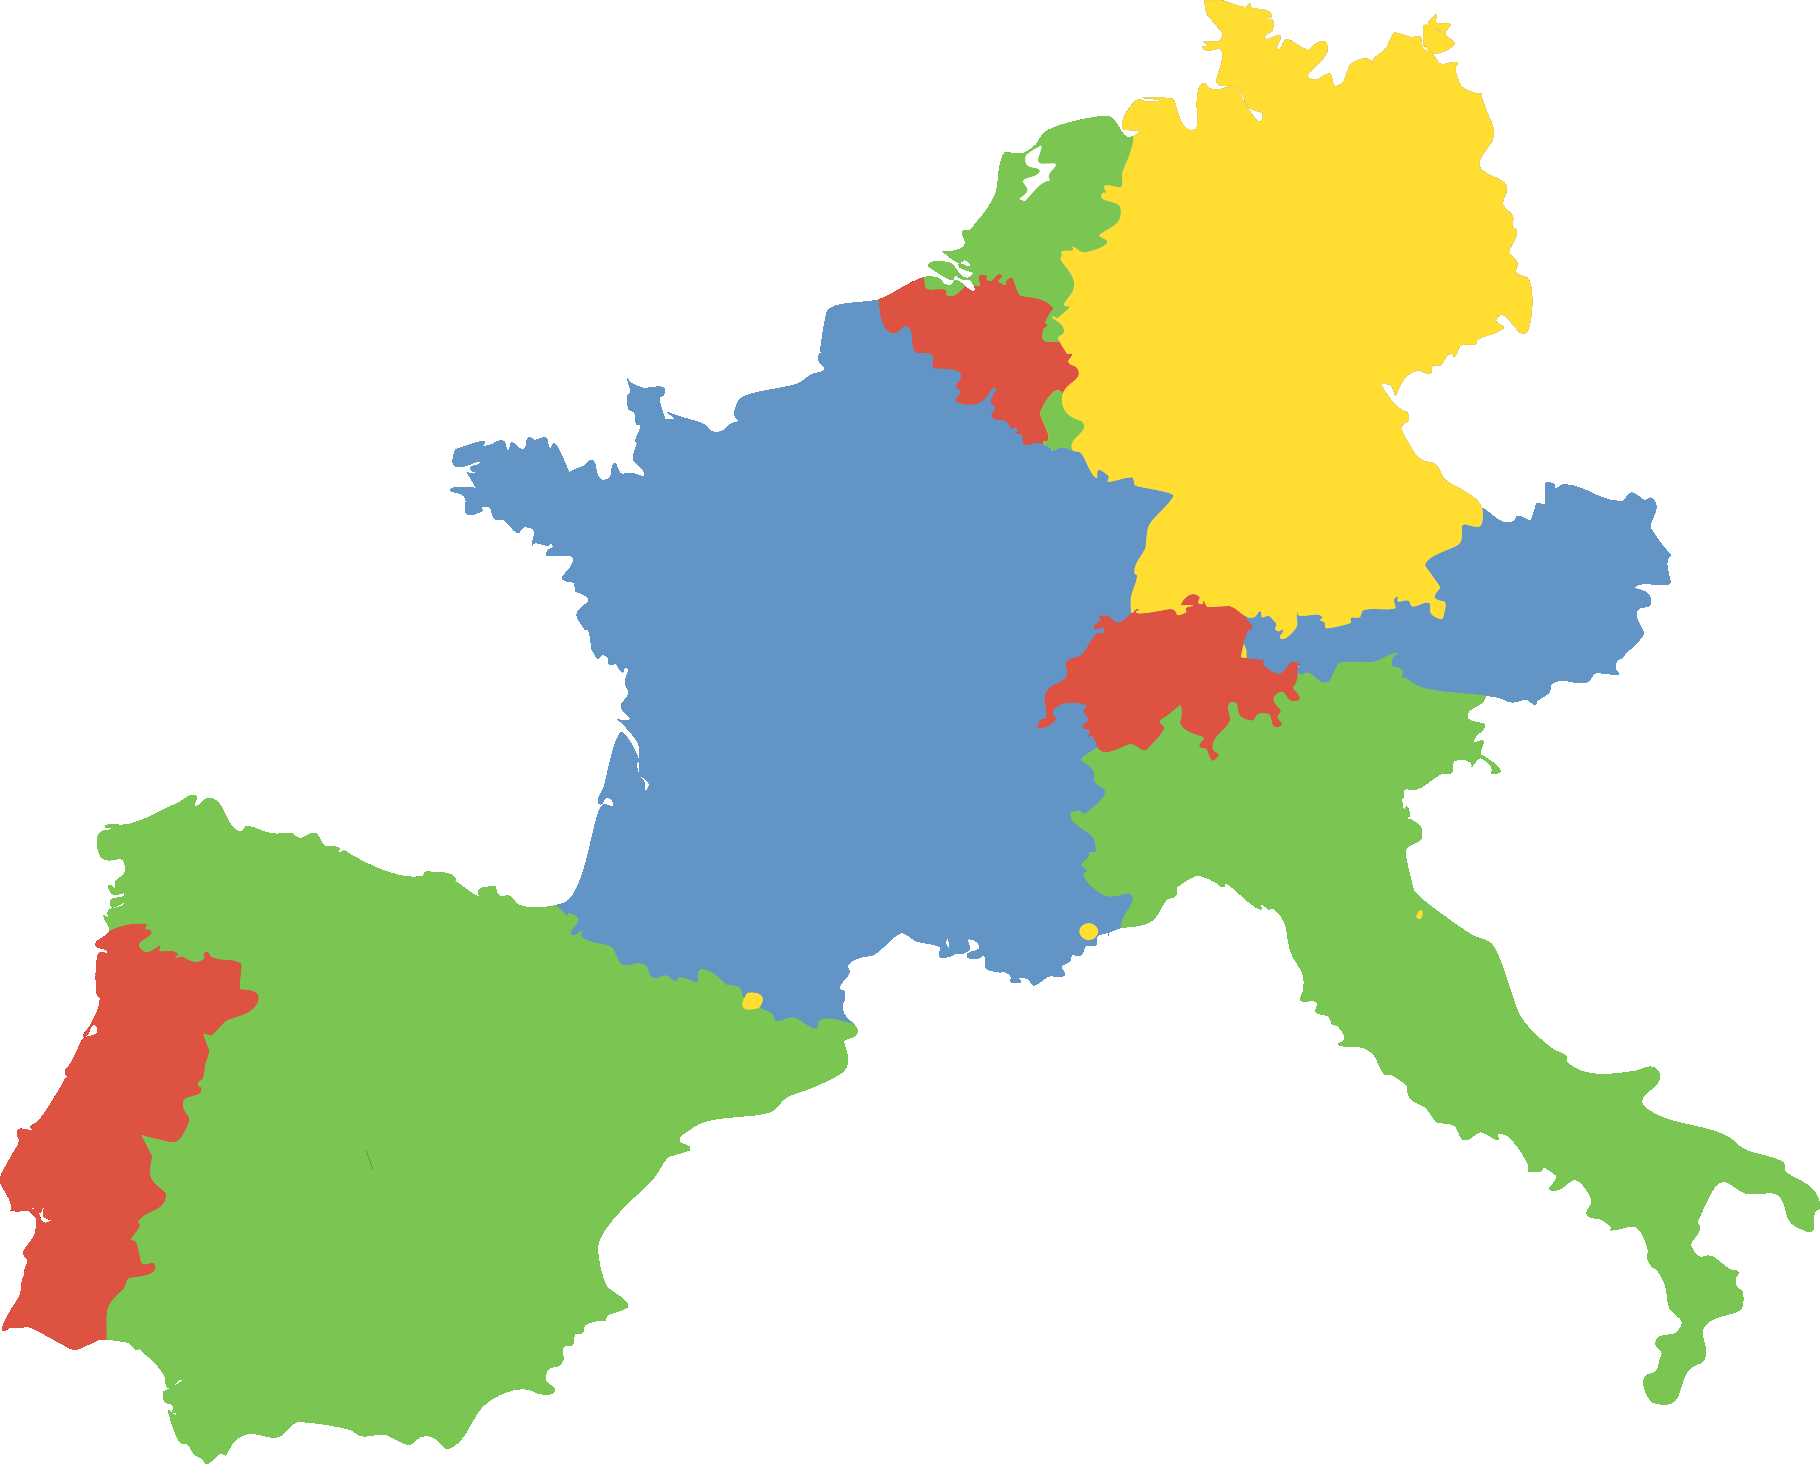
\includegraphics[width=.45\textwidth]{Carte}\qquad
\begin{tikzpicture}[scale=2.0]
\node[draw, circle,minimum size=.7cm,fill=j] (DE) at (3.042,2.736) {\scriptsize{DE}};
\node[draw, circle,minimum size=.7cm,fill=j] (AD) at (1.884,1.301) {\scriptsize{AD}};
\node[draw, circle,minimum size=.7cm,fill=b] (AT) at (3.568,2.019) {\scriptsize{AT}};
\node[draw, circle,minimum size=.7cm,fill=r] (BE) at (2.108,2.847) {\scriptsize{BE}};
\node[draw, circle,minimum size=.7cm,fill=v] (ES) at (1.296,1) {\scriptsize{ES}};
\node[draw, circle,minimum size=.7cm,fill=b] (FR) at (2.025,1.884) {\scriptsize{FR}};
\node[draw, circle,minimum size=.7cm,fill=v] (IT) at (3.042,1.111) {\scriptsize{IT}};
\node[draw, circle,minimum size=.7cm,fill=j] (LI) at (3.078,2.188) {\scriptsize{LI}};
\node[draw, circle,minimum size=.7cm,fill=v] (LU) at (2.409,2.507) {\scriptsize{LU}};
\node[draw, circle,minimum size=.7cm,fill=j] (MC) at (2.353,1.301) {\scriptsize{MC}};
\node[draw, circle,minimum size=.7cm,fill=v] (NL) at (2.460,3.185) {\scriptsize{NL}};
\node[draw, circle,minimum size=.7cm,fill=r] (PT) at (0.796,1) {\scriptsize{PT}};
\node[draw, circle,minimum size=.7cm,fill=j] (SM) at (3.568,1.371) {\scriptsize{SM}};
\node[draw, circle,minimum size=.7cm,fill=r] (CH) at (2.670,1.884) {\scriptsize{CH}};
\node[draw, circle,minimum size=.7cm,fill=r] (VA) at (2.536,0.851) {\scriptsize{VA}};
\path (DE) edge (NL);\path (DE) edge (BE);\path (DE) edge (LU);\path (DE) edge (CH);\path (DE) edge (AT);\path (DE) edge (FR);
\path (AD) edge (FR);\path (AD) edge (ES);
\path (AT) edge (CH);\path (AT) edge (LI);\path (AT) edge (IT);
\path (BE) edge (NL);\path (BE) edge (LU);\path (BE) edge (FR);
\path (ES) edge (PT);\path (ES) edge (FR);
\path (FR) edge (IT);\path (FR) edge (CH);\path (FR) edge (LU);\path (FR) edge (MC);
\path (IT) edge (SM);\path (IT) edge (CH);\path (IT) edge (VA);
\path (LI) edge (CH);
%  \path (2) edge[looseness=1.8,bend left=90] (5);
\end{tikzpicture}
\caption{Exemple de carte géographique et du graphe associé}\label{Carte}}
\end{figure}

Puisque les graphes que nous considérerons proviennent tous de cartes géographiques, ils satisfont aux propriétés suivantes :
%\begin{enumerate}
\begin{description}

\item[\textbf{Simple ·}] Un pays n'ayant pas de frontière avec lui-même, le graphe ne présente pas de boucle (c'est-à-dire d'arête retournant sur le sommet dont elle est issue). De même, une et une seule frontière peut exister entre deux pays (connexes) et il ne peut dès lors y avoir d'arêtes multiples entre deux sommets. On dit d'un graphe sans boucle ni lien multiple qu'il est \textit{simple} ;
\item[\textbf{Planaire ·}] Une frontière ne pouvant se restreindre à un seul point, les arêtes du graphe ne peuvent pas se croiser. De plus, quelque soit la projection utilisée, une carte peut toujours être représentée sur un plan, sans devoir introduire de troisième dimension. Dès lors le graphe associé est également restreint à un plan et un sommet ne peut être relié par un autre en passant \textit{au dessus} d'arêtes ou de sommets. Ainsi, le seul endroit où deux arêtes peuvent se rencontrer est en un sommet. On dit d'un graphe pouvant être représenté sur un plan de façon à ce qu'aucune arête ne se croise qu'il est \textit{planaire} ;
\item[\textbf{Connexe ·}] Tous les pays étant regroupés en un bloc unique (\textit{i.e.}~un continent), tous les sommets sont reliés les uns aux autres par des arêtes et on peut toujours trouver une succession d'arêtes (ce qu'on appelle un \textit{chemin}%\footnote{Lorsqu'on parlera de longueur de chemin et de chemin fermé, on sous-entendra par \textit{succession d'arêtes} qu'on ne passe jamais plus d'une fois par la même arête, quelque soit le sens de parcours.}
) qui relie n'importe quelle paire de sommets. On dit alors que le graphe est \textit{connexe}.
%\end{enumerate}
\end{description}
Tous les graphes que nous considèrerons par la suite seront simples, planaires et connexes. Pour éviter la lourdeur de répétitions continues, nous sous-entendrons ces hypothèses par la dénomination de \textit{graphe géographique}.

\section{Chaine de Kempe}

Dans ce qui suit, nous utiliserons abondamment la notion de \textit{chaine de \textsc{Kempe}}, à laquelle nous ferons référence en parlant simplement de \textit{chaine}. Une chaine de \textsc{Kempe} est un sous-ensemble bicolore connexe d'une carte coloriée. En terme de graphes, une chaine de \textsc{Kempe} est un sous-graphe connexe maximum dichromatique. Remarquons que ces «~chaines~» ne sont pas nécessairement linéaires et peuvent être des arbres ou comprendre des chemins fermés. Dans une chaine (par définition bicolore), on peut toujours échanger les deux couleurs sans que cela ne pose de problème dans le coloriage général de la carte (ou du graphe associé). On notera $\mathcal{C}_{ab}$ la chaine comportant le sommet $a$ et dont la seconde couleur est celle du sommet $b$, celui-ci ne faisant pas nécessairement partie de la chaine (on peut donc avoir $\mathcal{C}_{ab}\cap\mathcal{C}_{ba}=\varnothing$).

Par exemple, sur la Figure~\ref{Carte}, le Benelux forme une chaine verte-rouge que l'on peut noter de plusieurs façons : $\mathcal{C}_{\textsc{be}\cdot\textsc{nl}}=\mathcal{C}_{\textsc{lu}\cdot\textsc{pt}}=...$ . De même, Andorre, Monaco, la France, l'Allemagne, l'Autriche et le Liechtenstein forment une chaine jaune/bleue. Inverser les couleurs jaune et bleue au sein de cette chaine donne une coloration tout aussi valable de la carte et du graphe.

Dans le cas où la chaine $\mathcal{C}_{ab}$ contient à la fois le sommet $a$ et le sommet $b$ (\textit{i.e.} lorsque~$\mathcal{C}_{ab}=\mathcal{C}_{ba}$), on dira que la chaine $a$-$b$ est complète, ce que l'on notera~$\overline{\mathcal{C}}_{ab}$.
%On notera dans la suite du document $\overline{\mathcal{C}}_{xy}$ la chaine commune a «~x~» et «~y~», soit lorsque la $\mathcal{C}_{xy}$ = $\mathcal{C}_{yx}$. 
